\documentclass[letter:wpaper]{article}
\usepackage{isea}
\usepackage[pdftex]{graphicx}
\usepackage{times}
\usepackage{helvet}
\usepackage{courier}
\usepackage[numbers]{natbib}
\pdfinfo{
    /Title (Art as Technology)
    /Author (Kynan Stewart Hughes)
}
% The file isea.sty is the style file for ISEA 2025 proceedings.
%
%\title{Art as Technology v1.0.1}
\title{Art as Technology}
% \author{Author: Anonymous\\
% School: Anonymous\\
% Institution: Anonymous\\
% Location: Anonymous\\
% Email: Anonymous\\
\author{Kynan Stewart Hughes\\
Creativity and Cognition Studios\\
University of Technology Sydney\\
Sydney, Australia\\
kynan.s.hughes@student.uts.edu.au\\
\newline
\newline
}
\setcounter{secnumdepth}{0}

\begin{document} 
% Setting the default tolerance level
% \tolerance=200
% Setting a high tolerance level
% \tolerance=10000
% Some more drastic measures for hbox issues
% \emergencystretch=4em
% \raggedright
\maketitle
\begin{abstract}

    This paper argues for the conceptualisation of art as a technology, exploring its implications through the lens of complexity. It challenges the traditional partitioning of art and technology, proposing that art is a codifying system that dislocates objects and materials from their original functions and meanings, and encodes them with new affective potential. In other words, it is a kind of technology that programs our capacity to attribute affective potential to objects. The analysis suggests that rethinking art as a form of technology has the potential to expand the creative possibilities for artists working with emerging technologies and offers a pathway to reconsidering our relationship with our technologies. The conclusion invites artists who work with emerging technologies to explore an ethical mode of crafting that foregrounds interdependence and complexity.

\end{abstract}

\keywords{Keywords}

Art, technology, complexity, aesthetics, affect, information, craft, systems, emergence, meaning, constraints, coarse–graining

\section{Introduction}

    Over the last 80 years, the concept of complexity has evolved into a meta-theory, which posits that almost everything can be viewed as a complex system comprised of nested complex systems, each interacting within and across blurred, overlapping boundaries with other systems. Everywhere we look, we see things interacting in ways that would have been impossible to predict, and when we look more closely, we find that the things themselves are emergent approximations of interactions between fleetingly stable regularities in a shifting and chaotic flow. Nothing exists in isolation; everything is interconnected, transient, and contingent. All is process.

    Over the last several decades, the development of scientific theories of complexity, including Chaos Theory, Dynamical Systems Theory, and Complex Adaptive Systems Theory, constitute a paradigm shift away from simplistic, clockwork models and the search for universal laws, and towards a view that embraces unpredictability, interdependence, and emergence \citep{StengersOrdrOtOfChs1984}. The ancient Western tradition of process philosophy \citep{SeibtStnfrdEncyclpdPrcssPhlsphy1974} has been invigorated by this shift, contextualising knowledge from science and mathematics within a sophisticated materialist ontology.
    
    This paper draws on both scientific theories of complexity and theories of art and of technology influenced by process philosophy. It is an experiment conducted at the boundary between art and technology which has implications, especially, for artists who work with emerging technologies.
    
    It starts from an idea only rarely \citep[pp.74–75]{SauvagnarguesArtmchns2016} and fleetingly \citep[p.202]{ZepkeOSullivanDlzCntmprryArt2010} articulated – that art is a technology. We may have an edge against this idea. It might feel risky, as if art needs to be protected from such a move. Perhaps we fear that thinking of art as a technology will destroy the special qualities of art and reduce its value as a practice. This paper explores the potential for another outcome in which the idea of art as a technology leaves art intact but more connected, and opens new possibilities for how we make sense of technology as a field of practice that includes artmaking. 
    
    “Art as technology” is proposed as a kind of heuristic for creative technologists of all kinds, opening a space of possibility for crafting differently with art and with technology.

\section{Technology: A Programming of Perceived Regularity for a Purpose} 

    According to Brian Arthur a technical object is always “a phenomenon captured and put to use.” \citep[p.53]{theNatureOfTechnology2009} Put another way, a technology is “a programming of phenomena for a purpose.” \citep[p.53]{theNatureOfTechnology2009}. This distillation holds for the full range of diverse technologies, contemporary and historical. Phenomena don't have to be physical phenomena like fire or electricity. They may be “behavioural or organisational ‘effects’” \citep[p.55]{theNatureOfTechnology2009} or “truism[s] of nature” \citep[p.45]{theNatureOfTechnology2009}.

    \subsubsection{Coarse Graining}
    
    We can deepen Arthur's definition of technology by applying Jessica Flack's concept of \emph{coarse graining} in place of “phenomena”. According to Flack, coarse graining occurs when a subsystem with apparently emergent properties is treated as a single entity by components of the system for predictive purposes. Coarse graining is a way for components of complex systems (like people) to treat other elements the system that works but ignores many of the details. It is a “lossy but true” \citep[p.4]{FlackCrsGrnng2017} strategy.
    
    All apparent phenomena are the result of coarse graining. Coarse graining is “how adaptive systems identify regularities in evolutionary or learning time and use these perceived regularities to guide behaviour." \citep[p.2]{FlackCrsGrnng2017}. It is happening all the time in every system, from coral reef formation \citep[p.61]{FlackEtAlTmsclsSymmtryUncrtnty2013} to the way monkeys establish social hierarchy \citep{FlackCntxtMdltsSgnlMnng2007}.

    Coarse–graining describes how emergence happens – or at least something about its necessary conditions. In science, a property like temperature emerges, through processes that include coarse–graining, from interactions between physical substances, people measuring, devices, systems of measurement, and the environment \citep[p.4]{FlackCrsGrnng2017}. A distribution of relative status ‘scores’ in a monkey group emerges from a system of signalling interactions between individual monkeys and the perception of those signals by the group \citep{FlackCntxtMdltsSgnlMnng2007}. Undulations in the ocean floor transform into coral reefs as particles collect and aggregate, generating favourable conditions on which complex structures can form \citep[p.61]{FlackEtAlTmsclsSymmtryUncrtnty2013}.
    
    We might say then, that a technical object is a programming of \emph{perceived regularity} for a purpose.

    \subsubsection{Example: Money}

    Money is a technology because it depends on a perceived regularity of human behaviour, which is the trust people put in tokens of value.

    \begin{quote}
        The monetary system makes use of the “phenomenon” that we trust a medium has value as long as we believe that others trust it has value and we believe this trust will continue in the future. \citep[p.55]{theNatureOfTechnology2009}
    \end{quote}

    We have established a general definition of technology that can be applied to all technical objects. In the next section, we can experimentally apply this definition to art objects. First, we need to decide what art is – or, rather, we need to be clear about which of the overlapping ideas of art we mean when we say “art”.

\section{Art: A Technology That Encodes Affective Potential Into Objects}

    \subsubsection{The Aesthetic Regime}

    Jacques Rancière has called the currently dominant idea of art in our Westernised global context, the \emph{aesthetic regime}. It is not a single coherent paradigm, but a “plurality” of “frequently different, and sometimes contradictory, ways of thinking” \citep[p.8]{RanciereMdrnTms2022} about art organised around the idea of aesthetic experience.
    
    The aesthetic regime emerged at the end of the eighteenth century with Emanuel Kant's \emph{Critique of Judgement} and some other key texts that followed it \citep[pp.23–24]{RancierPltcsOfThAsthtcs2004}. Kant's radical break was to propose that the essence of an art object lies in its capacity to be experienced without concept. With the clarity of hindsight, we can see as Rancière did, that it is the separation of sense–as–in–sensation from sense–as–in–making–sense which created our current situation in which the effectiveness of an artwork, the very thing that makes an object art, is “a paradoxical kind of efficacy that is produced by the very rupturing of any determinate link between cause and effect.” Artworks need not make sense. “It is precisely this \emph{indeterminacy}\footnote{
        My emphasis.
    }”, he said, “that Kant conceptualized when he defined the beautiful as ‘what is represented as an object of universal delight apart from any concept’”. \citep[p.51-52]{RancierThEmncptdSpcttr2009}

    The identity of an artwork as an artwork is organised solely around aesthetic experience. This constraint is the origin of art's autonomy within Modernity and the source of all possibility with respect to how art objects can interact with other aspects of Modernity – including all potential for generating meaning or taking political action, for example. All distinctions and differences within the idea of art operate within the aesthetic regime. Ideas about Modern and Post–Modern art, for example, are contradictory strategies for taking meaningful action within the aesthetic regime \citep[p213]{ZepkeSblmArt2017}. Art which is anti–aesthetic is operating within the aesthetic regime in a way that is self–consciously critical of it. Conceptual art is art that invites us to consider the aesthetic potential of ideas.

    The aesthetic regime enables objects created for purposes other than aesthetic appreciation to be experienced as art. As Marcel Duchamp proved in 1917 when he entered a urinal into an art exhibition, and as has been proven many times since by practitioners of the style known as Contemporary Art for whom the readymade is a key strategy, there is nothing in the world that cannot be made into a work of art by the simple act of declaring it to be one. A transfiguration, or dislocation, occurs when an object is brought into the aesthetic regime. The object is no longer understood in terms of its original function or purpose, but as an object of contemplation within the aesthetic regime. “The aesthetic regime”, as Rancière put it, “asserts the absolute singularity of art and, at the same time, destroys any pragmatic criterion for isolating this singularity.” Literally anything can be art.
    
    The aesthetic regime is a codifying system\footnote{
        The scientific term “complex adaptive system” is synonymous with the term “assemblage” for process philosophers. In Manuel DeLanda's Assemblage Theory, “coding refers to the role played by special expressive components in an assemblage in fixing the identity of a whole. The two best-known expressive components with a specialised function are chromosomes and languages” \citep[p.22]{DeLandaAssmblgThry2016}. In the aesthetic regime, the expressive components are art objects and styles, tropes like “the nude”, gallery systems, the language of art theory, et cetera.
    } that dislocates objects from their original functions and meanings. The “dissensual operation” of creating an artwork, for example by working materials into forms, by organising sounds in certain ways, by setting the state of pixels on a screen, by isolating and performing specific movements with our body, or by appropriating a ready–made object, “transforms a given form or body into a new one.” \citep[p.54]{RancierThEmncptdSpcttr2009}.

    Having established that the terms “artworks” and “art objects” apply to materials and objects that are encoded by the aesthetic regime, we can think about how the idea of technology as {\emph{the programming of perceived regularity for a purpose}} might apply to them. A question immediately arises: what perceived regularity do art objects capture?

    \subsubsection{Affect}

    The concept of \emph{affect}, which comes from Deleuze and Guattari via Brian Massumi, is a way of thinking about how things affect other things and are affected, including our bodies and minds, in the complex interconnected systems of material reality. Affect is a kind of intensive, interactive event. It is human and inhuman, organic and inorganic. It is the way that we and things are moved by the world and each other. It is a pre–cognitive, pre–linguistic, pre–conscious event during which the world emerges into existence. Perceived regularities happen when affect happens.
    
    In a reality that consists entirely of unfolding processes, objects are processes that stay still long enough to be noticed. Objects come into existence for us through processes of coarse–graining, which are material, cognitive and social. Objects are \emph{slow variables} – that is, they are “macroscopic states that [...] change slowly with respect to the underlying dynamics generating the state” \citep[p.61]{FlackEtAlTmsclsSymmtryUncrtnty2013}. Once called into existence, objects seem to embody the affective properties and capacities – the \emph{estimated regularities} \citep[p.9]{FlackCrsGrnng2017} – that caused them to appear. This is especially so for art objects because it is their primary function.

    For Kant, the range of aesthetic experience as it pertains to artworks was limited to the experience of beauty. These days, an exclusive focus on beauty when it comes to aesthetic experience and art, seems like an unnecessary limitation to put on aesthetic experience, and on art \citep[pp.121–122]{HighmoreBttrAftrTst2010}. The recent move to equate aesthetic experience with affect is a shift away from the idea that normative experiences of beauty are better than other experiences with artworks, and that artworks are moral lessons, and towards the messy reality of material processes. It contextualises aesthetic experience in a complex ecology of affect. Art is increasingly about “complex affective and intensive exchanges, situated in the broader ecology of the world.” \citep[p.155]{HighmoreBttrAftrTst2010}

    Humans are particularly good at attributing affective regularity to objects \citep{FristonThFrEnrgPrncpl2010} \citep{DeaconTheSymbolicSpecies1998}, and this is the perceived regularity that art objects capture. We see faces in clouds, spirits in trees, and stories in rocks. Art is a system of coding that exploits this capacity. The codes of the aesthetic regime govern the production, distribution, and reception of art objects. Through a process of becoming art, objects become slow variables packed with potential affect, like batteries holding a charge.

    The affective charge of an art object can consist of any combination of qualities – strong, weak, sensorial, semantic, abstract, pleasant and unpleasant et cetera. It can be a sense of the beautiful, or it can involve concepts and feelings that are more difficult to pin down. It can, like a Patricia Piccinini sculpture, strobe between incompatible affective states, such as the cute and the grotesque. Like a readymade, it can call attention to the affective charge of art itself.

    In summary: art is a kind of technology that encodes – or \emph{programs} – our capacity to attribute affective potential to objects. The terms “artworks” and “art objects” apply to materials, even pre–existing objects, programmed by the aesthetic regime with new affective potential.
    
\section{Meaning as Purpose}

    Having highlighted the way art functions technically, the question of \emph{purpose} remains. If we are to continue experimentally thinking of art as a technology, we must consider whether the nature of purpose with respect to art objects is different enough from the nature of purpose with respect to technical objects to warrant separating artmaking as a set of practices from technology as a different set of practices.
    
    \subsubsection{Meaning as Context}

    Arthur Danto said that artworks are “embodied meaning” \citep[p.125]{DantoEmbdMnngs2007}, and meaning is a useful way to think about the purpose of art objects as long as we are clear about the meaning of “meaning”.
    
    In saying that art objects embody meaning we run the risk of conflating or confusing two different uses of the word “meaning”. Manuel DeLanda has pointed out that the words “meaning” in the expressions “this word has a meaning” and “this life has a meaning” are two entirely different words, and that “using them as if they were the same word can lead to erroneous conclusions \citep[pp.40–41]{DeLandaCsltyAndMnng2018}. It is probably better to be more specific and say that art objects embody \emph{context} because context is the origin of the kind of meaning we mean when we talk about art. Massumi has said, “meaning is [...] a network of enveloped material processes” and, quoting Deleuze and Guattari, “‘A thing has as many meanings as there are forces capable of seizing it.’” \citep[p.10]{MassumiAUsrsGdTCptlsmAndSchzphrn1992}.

    Context is an important concept because complex systems always exist in overlapping and nested relationships with other systems\footnote{
        Context is roughly synonymous, in scientific terms, with the control space of a system \citep[p.130]{DeLandaAssmblgThry2016}, which is integral to the probability space of the system's possible states – or, the “state space” of the system.
    }. Art objects are, like most things, complex systems. In order to think about the way art objects fulfil their purpose of embodying meaning it will be necessary to examine how they function in relation to their context.
    
    \subsubsection{Epiphenomenal Objects with Indeterminate Meaning}

    Jason Hoelscher has pointed out that art objects are epiphenomenal, like rainbows \citep[p.17]{HoelscherArtAsInfrmtn2021}. It is always possible to see how they are the result of some other phenomena. The materials from which they are made are always visible, and yet the artwork exists somehow separately from these materials. An art object is made, in a way, out of its own \emph{artness} that emerges from the combination and arrangement of existing objects and materials \citep[p.2]{HoelscherThPtcsOfPhsSpc2014}. Epiphenomena like rainbows and art objects are compelling. They grab our attention by virtue of their complex, contingent mode of existence \citep[p.18]{HoelscherThPtcsOfPhsSpc2014}. 
    
    In Hoelscher's formulation, art objects are \emph{indeterminate} because they are, as Kant suggested, “purposive without a purpose” \citep[p.57]{KantCrtqOfJdgmnt}. Kant's formulation is reinterpreted by Hoelscher to mean “not that art lacks purpose, but that art's purpose is contextually complex and indeterminate, and so remains open to transformation, [...] many layered, and multidimensional.\citep[p.25]{HoelscherThPtcsOfPhsSpc2014}

    Objects instantiated as artworks remain indeterminate in that their meanings are not fixed – they are always susceptible to shifting context. The shifting meanings attributed to art objects over time and in different contexts are “a series of attractor basins in possibility space” \citep[p.4]{HoelscherThPtcsOfPhsSpc2014}. Being unfinalisable and open, an artwork draws the viewer toward possible interpretations while nonetheless preventing a fixed, final understanding. A swarm of interpretations are possible but never definitively attained. \citep[p.12]{HoelscherThPtcsOfPhsSpc2014}

    \subsubsection{Difference as Information}

    The resolution of meaningless disparity into meaningful difference is the process by which all things come into existence. It is everywhere and always a wildly creative event that results in an exponentially more vast field of potential for meaningful action – a huge increase in capacity to affect and be affected. Hoelscher has invited us to consider, for example, the evolution of eyes from, perhaps, light–sensitive areas on an organism's surface. These areas eventually become sensitive enough to allow the creature to perceive a consistent difference in the input signal from different eyes. In the macro–scale equivalent of a quantum shift, a three dimensional universe comes into existence \citep[p.5]{HoelscherArtAsInfrmtn2021}.

    It has been suggested that information is as fundamental a concept for contemporary physics as energy was for classical physics\footnote{
        “[...] every item of the physical world has at bottom [...] an immaterial source and explanation; [...] all things physical are information-theoretic in origin and this is a participatory universe.” \citep{WheelerInfrmtnPhscsQntm2018}
    }. Hoelscher has blended Claude Shannon's Information Theory with Gilbert Simondon's idea of information arising from meaningless disparity as emergent, meaningful difference. He defines information as the “relational operation of difference that intensifies or generates a context” \citep[p.6]{HoelscherArtAsInfrmtn2021}. In embodying meaning, art objects are tapping into the generative power of the universe itself. They function as “differentially complex” \citep[p.74]{HoelscherArtAsInfrmtn2021} objects making information available that is otherwise hidden in plain sight as apparently disordered, entropic chaos. In other words, they organise information about their context, making it available as meaning.

    \subsubsection{Examples: Robert Morris and Marcel Duchamp}

    \begin{figure}[h]
        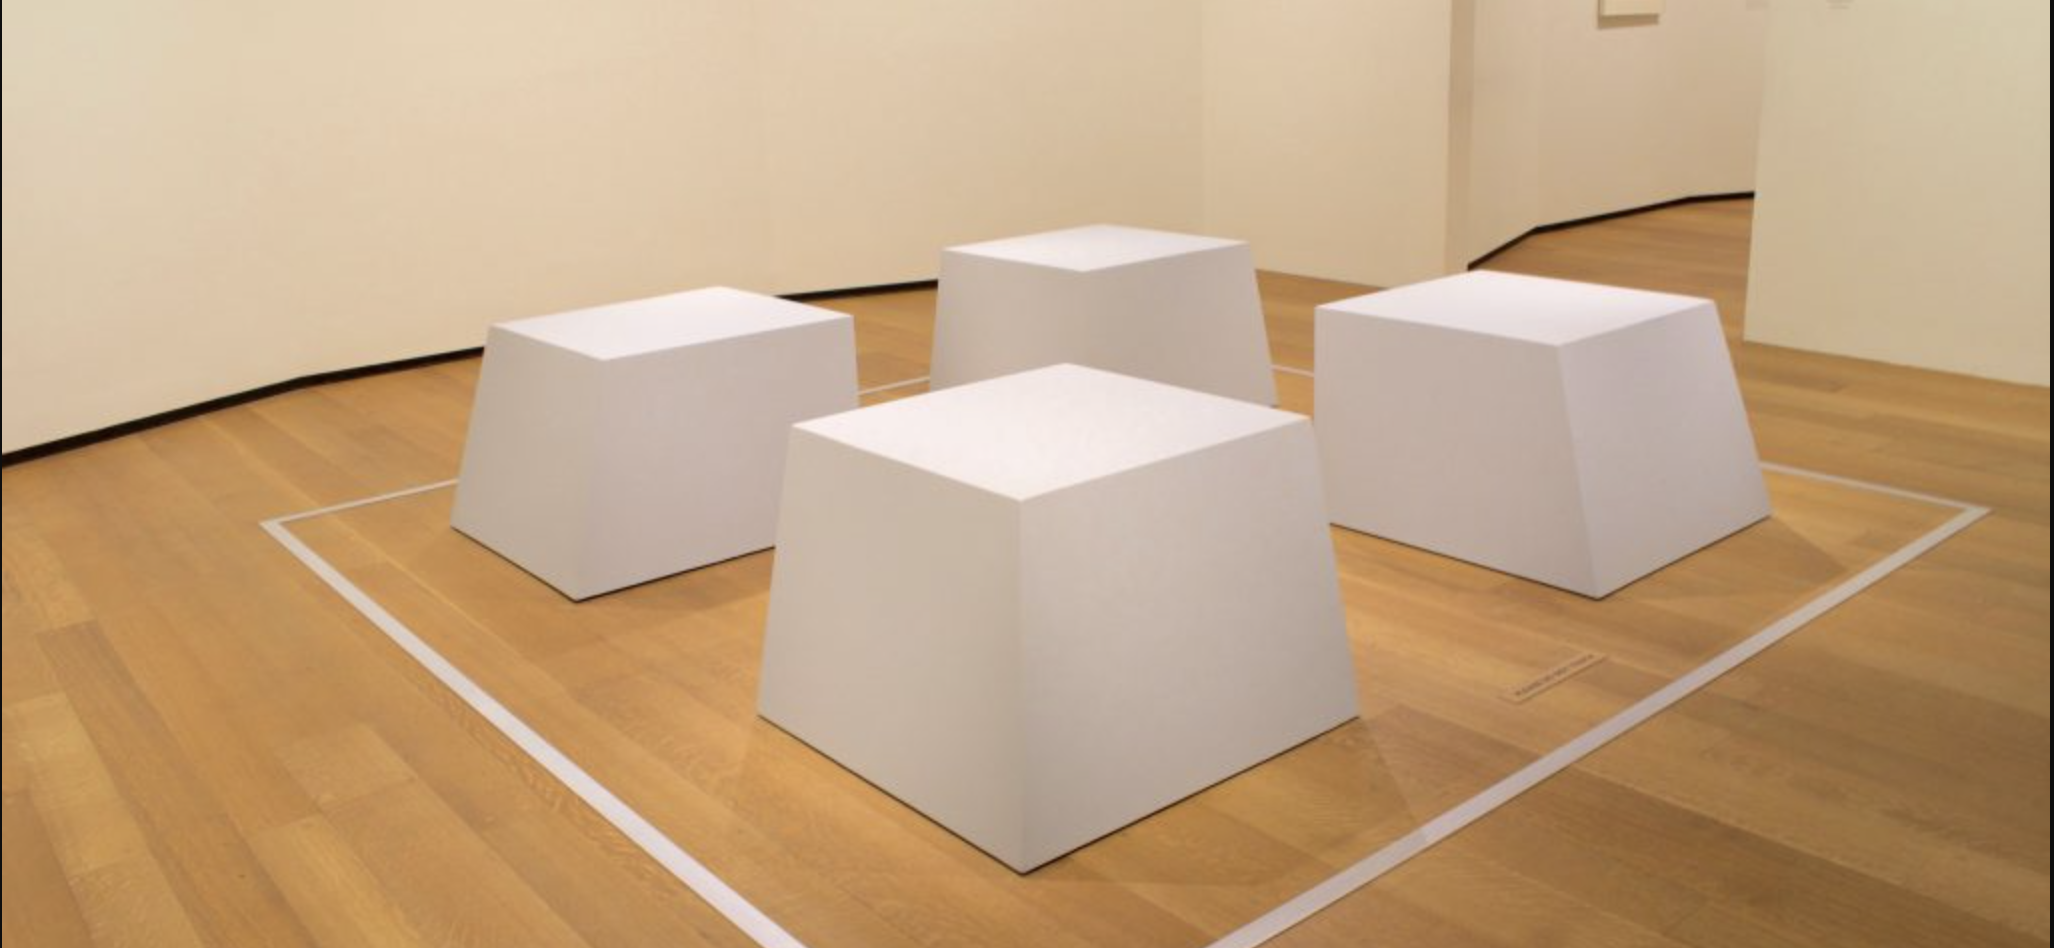
\includegraphics[width=3.31in]{robert-morris-cubes.png}
        \caption{Robert Morris, American, born 1931. \emph{Untitled (Battered Cubes)}, 1966. Painted Fibreglass (4 Units). Source: https://www.theextravagant.com/lifestyle/art-culture/when-art-is-not-about-art-but-about-you/.}
        \label{fig:robert-morris-cubes}
    \end{figure}

    For an example, Hoelscher uses the hyper minimalist sculptures of Robert Morris, which are simple grey cube–like forms placed directly on the floor of a gallery (Figure~\ref{fig:robert-morris-cubes}).

    \begin{quote}
        By giving the viewer so little to look at, Morris [...] directs the flow of attention away from the object itself and toward the object's relations with the gallery space, with the changes of light and shadow over time, and with the viewer's field of experience as an experience in and of itself. Accordingly, with the severe reduction of the work's surface qualities, internal differentiations, particularity, and variability, the artwork and its local situation fold into one another – a direct ingression of the differential information object into the space of lived experience. \citep[p.78]{HoelscherArtAsInfrmtn2021}
    \end{quote}

    \begin{figure}[h]
        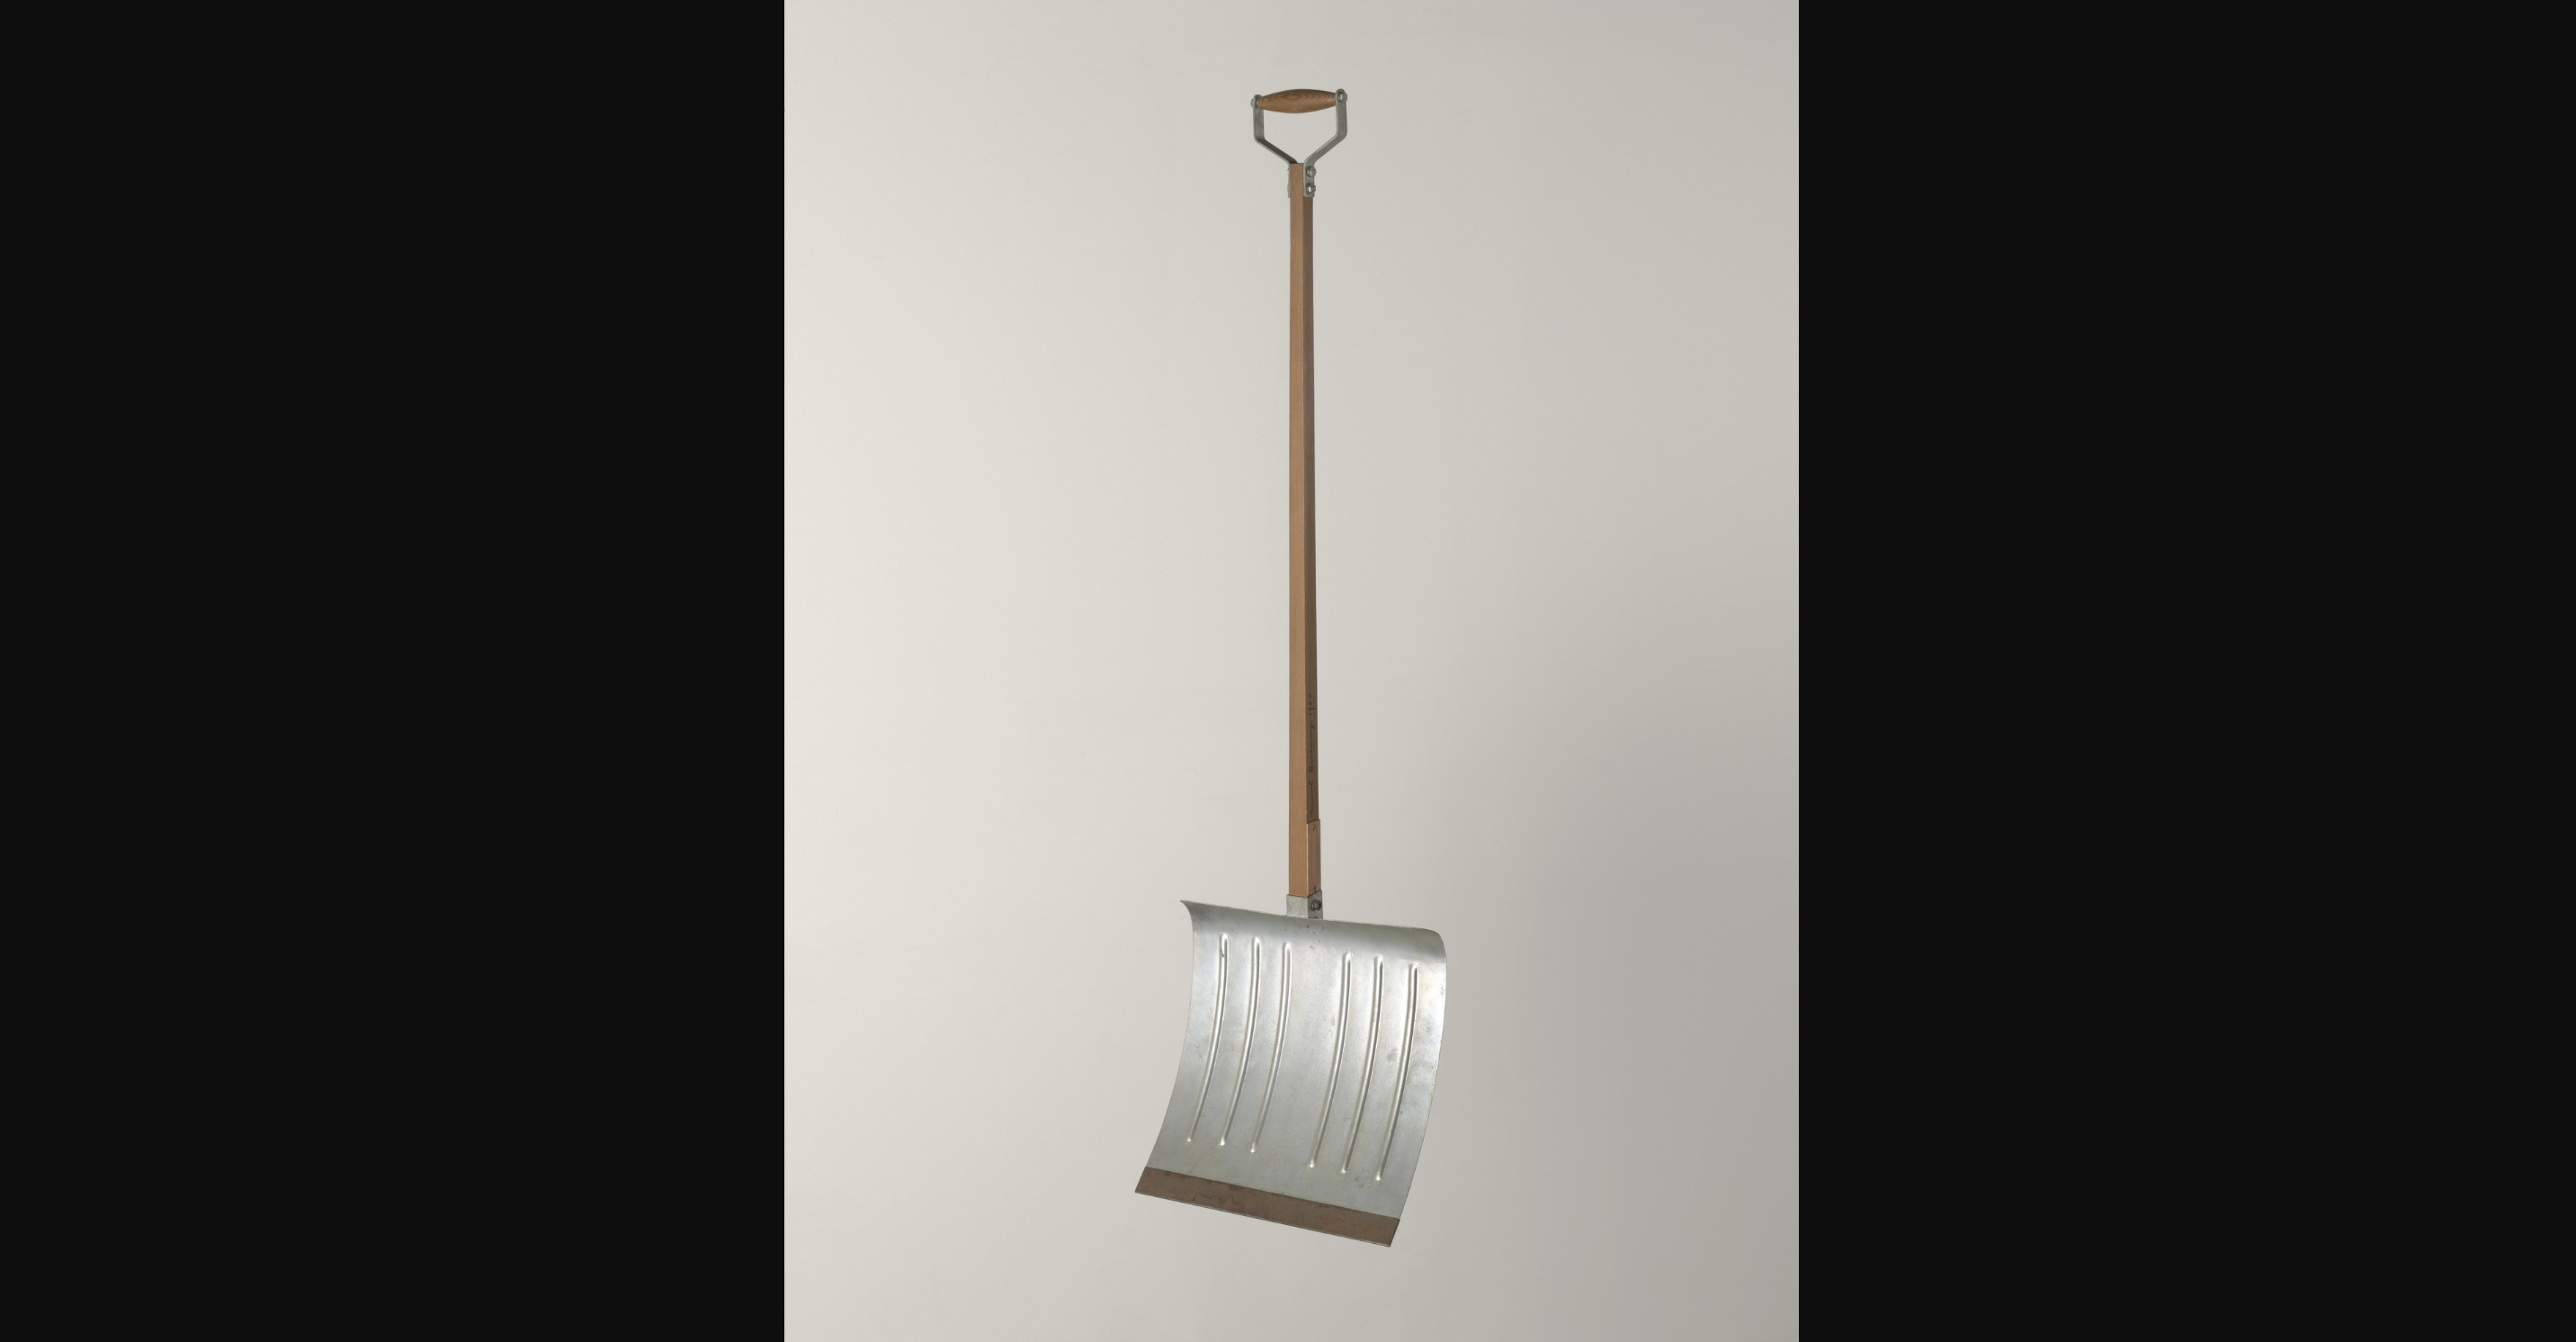
\includegraphics[width=3.31in]{snow-shovel.png}
        \caption{Marcel Duchamp, \emph{In advance of the broken arm}, 1964 (fourth version of the lost 1915 original). Ready–made, snow shovel. New York, Museum of Modern Art. Source: https://www.artesvelata.it/marcel-duchamp/.}
        \label{fig:snow-shovel}
    \end{figure}

    Another example is a Duchamp readymade \emph{In Advance of the Broken Arm} (a snow shovel) (Figure~\ref{fig:snow-shovel}).

    \begin{quote}
        [...] the readymade's enfolding of object and idea activates (and is activated by) a wide–ranging network of differential tensions between the object and its context, and between cultural, historical, and artistic expectations regarding shovels, artworks, and the application of artistic skill [...] \citep[p.187]{HoelscherArtAsInfrmtn2021}
    \end{quote}

    This is nothing we haven't heard before with respect to a Duchamp readymade. What is interesting is that the functioning of both the Morris sculpture and the readymade, their embodying of meaning, is described in terms of existing information reordering around epiphenomenal art objects. The Morris sculpture reorders information around the object's relation to the gallery space, light and shadow, and the viewer's experience. The Duchamp readymade reorders information around the object's relation to the history of art, the history of shovels, and the history of Duchamp's own work. The reordered information is different, but the process is the same.

    \subsubsection{Enabling Constraints}

    Alicia Juarrero's concept of \emph{enabling constraints} is useful as a way to think about meaning as context because it gives artists something to work with.
    
    Juarrero has identified two types of constraints that define the probability space of complex systems: context–free constraints and context–sensitive constraints. In terms of information, both types of constraints are necessary for reducing randomness in order to separate information from noise but, she says, only context–sensitive constraints enable signals that convey meaning. While both types of constraints function by limiting possibilities, context–sensitive constraints also create possibility by connecting a message/information system that is initially defined by context–free constraints with the complex systems in which it is embedded.
    
    Context–sensitive constraints create new dimensions of possibility by connecting the system with the state–spaces of other systems. Like coarse–graining, context–sensitive constraints are a way to explain emergence \citep[p.193]{JuarreroThSlfOrgnstnOfIntntnlActn2004} \citep[p.240]{JuarreroCsltyAsCnstrnt1998}.

    For example, a lighthouse is physically constrained to having only two possible states – it can only blink on and off. Because it is seen within the network of contextual relationships that include navigation, a sailor can understand the flashes of light as meaning "Land!". Signals subject to contextual constraints refer to the contextual web (temporal and spatial) in which that particular signal or event is embedded. The information such signals or processes carry is of the organisation of the network \citep[p.237]{JuarreroCsltyAsCnstrnt1998}
    
    If we want to add more meaning to the flashing signal, we impose more constraints on it. For example, Morse code puts strict constraints on a simple on/off signal like a flashing light – every combination of flashes must amount to one of the 54 symbols in the code – but the signal information is suddenly of the organisation of a much larger network of potential meaning – of language.

    The concept of enabling constraints gives us something to grab onto and manipulate. The meaning of an art object emerges from the constraints that connect it with a broader network of things and events. The meaning of an art object is the information it carries about the organisation of this network. This leads to an interesting heuristic for artists (the articulation of a control system perhaps): if we want to add more meaning to an art object, we need to impose more constraints on it.

    \subsubsection{Example: \emph{Algorithm}}

    \begin{figure}[h]
        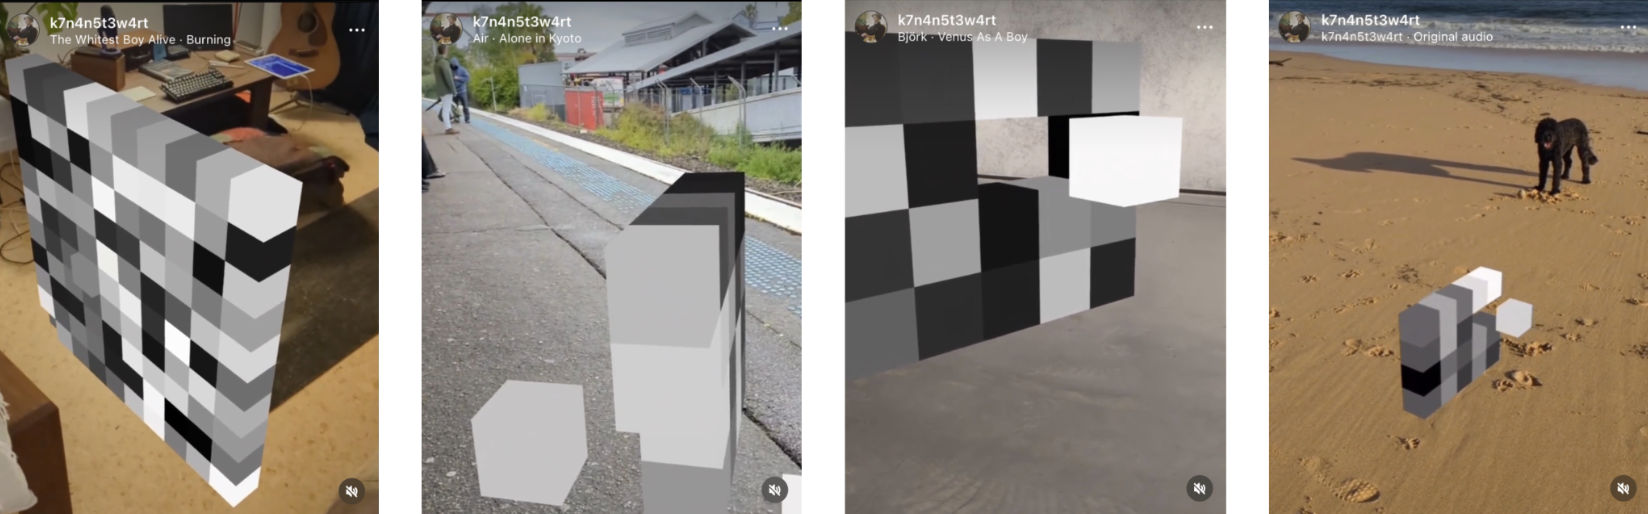
\includegraphics[width=3.31in]{bubble-sort.png}
        \caption{Some instances of the \emph{Algorithm} series, 2020. \copyright Respect Copyright.}
        \label{fig:bubble-sort}
    \end{figure}

    A simple example is an experiment of my own: a series of augmented reality sculptures called \emph{Algorithm} (Figure~\ref{fig:bubble-sort}), which rely on a limited set of constraints for their meaning.
    
    To start, some simple constraints define a limited possibility space that gives the pieces in the series a minimalist stylistic consistency. Each piece in the series is a single wall of greyscale blocks. The number of rows and columns in the wall is variable, as are the dimensions of the blocks, but they all look recognisably similar. The constraints that produce stylistic consistency are not especially meaningful, but they couldn't be described as “context–free” because they locate the work within a certain tradition of stylistic minimalism\footnote{
        It is interesting to consider the possibility that Juarrero's “context free” constraints are simply constraints that are not currently meaningful. A stylistic constraint, for example, if the viewer is not familiar with the style, would be effectively context–free.
    }.
    
    Each piece in the series depicts a different sorting algorithm from the early history of computing. The blocks animate, sorting themselves from lightest at the bottom to darkest at the top, then randomly scatter, and the sorting process starts again. The blocks move according to the the algorithm they represent. The particular sorting algorithm functions as a meaningful, or “enabling” constraint, because the qualitative difference between the pieces is entirely derived from the way the blocks move. Each algorithm is experienced as having a markedly different quality, and it is possible to recognise the particular algorithm from watching the way the blocks move. This series explores the resonance these primitive algorithms have in an era in which their contemporary descendants organise large portions of our lives. Their simple, human–made quality and human scale reference the craft that lies behind information technology.

    \subsubsection{Non–art purposes}

    The purpose of an art object is to embody meaning, but we might call this the ‘art purpose’ of an art object because art objects always have other, ‘non–art purposes’. For example, the art purpose of a painting may simply be to evoke an affective experience of beauty, but at the same time it may confer status, be an investment, or start a revolution. If art objects have as many meanings as there are forces capable of capturing them \citep[p.4]{DeleuzeNtschAndPhlsphy2006}, then we might say the same with respect to their non–art purposes.

    The affective charge of an art object may derive, to some extent, from a non–art purpose, but is never reducible to it. There is always “contextual excess or remainder” \citep[p.252]{MassumiPrblsFrThVrtl2002}. In socially connected art, participatory art, and art that is made to be used (craft), for example, non–art purpose and art purpose are entangled. Incorporating non–art purpose into the meaning of an art object is a risky strategy, which is what makes it interesting.
    
    When art purpose and non–art purpose become confused in an artwork, it is the art purpose that suffers. This is particularly relevant for artists who work with emerging technologies because the non–art purposes of emerging technologies are exciting and not fully understood. The meaning of an art object that incorporates emerging technology is likely to be ambiguous because it is entangled with the non–art purposes.
    
	In the early 2000s, practitioners of locative art were criticised for their uncritical use of mapping and networked, location-aware, mobile technologies, as well as for their collaborations with industry. It was alleged that they lacked a structure of accountability and ethics, were ushering in a `society of control', and were turning the media-art conference circuit into a `shopping-driven [...] spectacle' \citep[p.358]{beyondLocativeMedia2006}. Locative art was described as a “technocentric fantasy” that “downplays [...] history” and “evades categories of embodied difference such as race, gender and class” \citep[para. 2]{questioningTheFrame2004}. Clearly the art purpose of locative art was being hampered by the artists' failure to account for the non–art purpose and potential inherent in these technologies. Today, as we grapple with the conjunction of rampant technology-fuelled capitalism, privacy issues and mass surveillance, the criticisms seem to have been validated. 

    The desire to do something useful with technology based art is also a risky move. Should the meaning of an art object become reducible, for the viewer, to a non–art purpose, it would have ceased to be an art object, as the next example, drawn from my own experience, shows clearly.

    \subsubsection{Example: \emph{FlowAttractor}}

    \begin{figure}[h]
        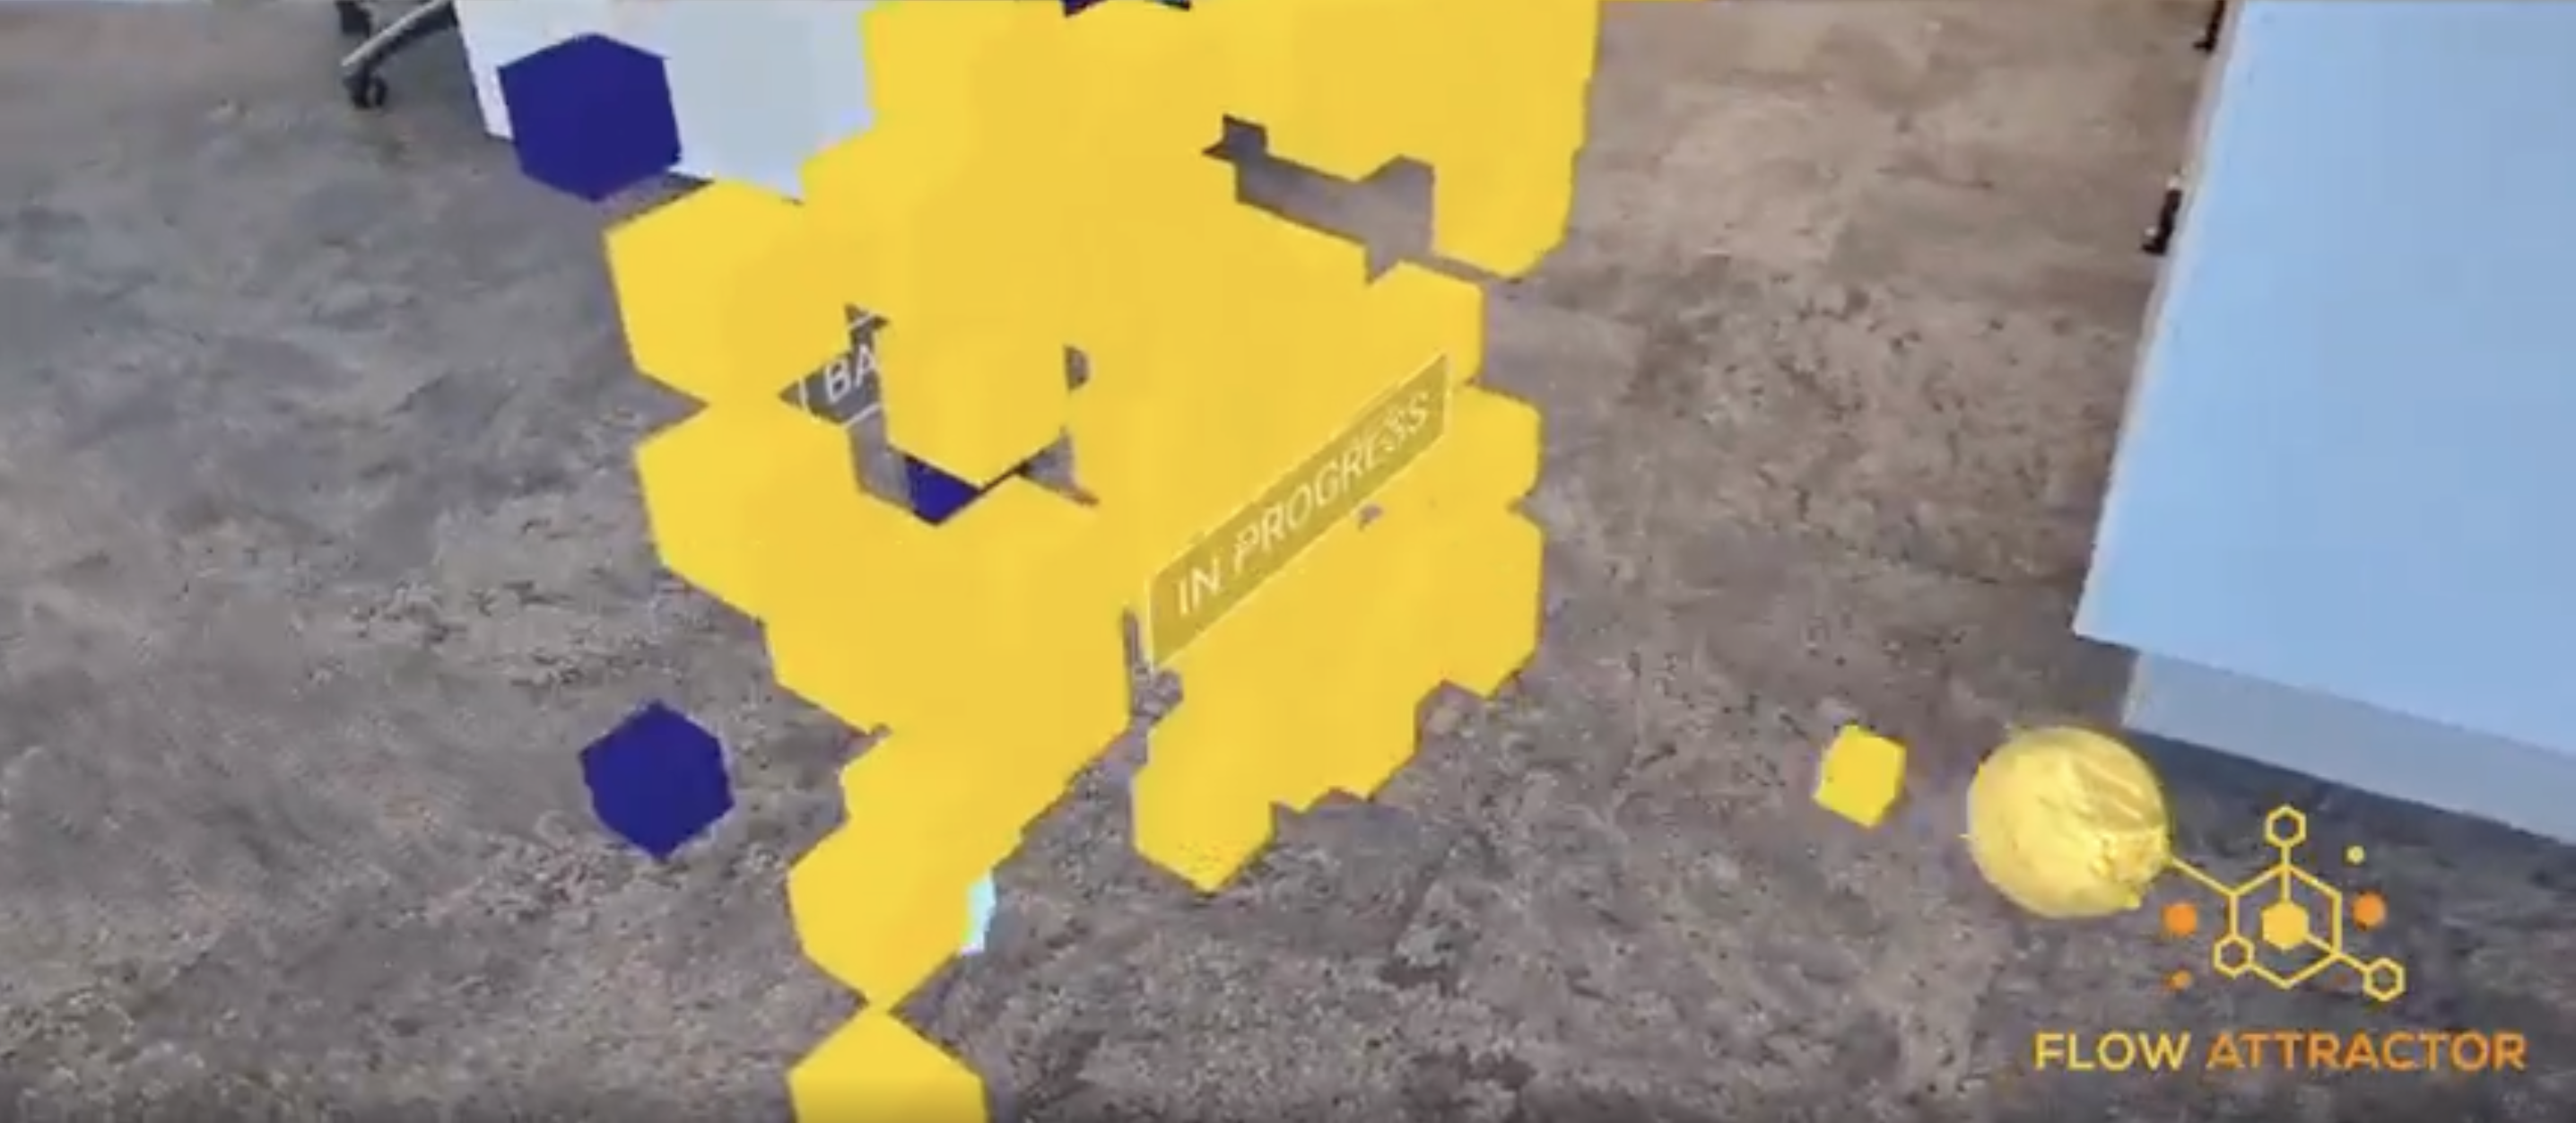
\includegraphics[width=3.31in]{flow-attractor.png}
        \caption{\emph{FlowAttractor} models complex workflows as flying cubes. \copyright Respect Copyright.}
        \label{fig:flow-attractor}
    \end{figure}

    In \emph{FlowAttractor} (Figure~\ref{fig:flow-attractor}), the flow of the blocks represents the otherwise invisible flow of work items through the software production system of a large organisation. The piece is an experiment to find out what can happen if an art–like object is integrated into a business context. Its non-art purpose is to catalyse an awareness of the effects of making small decisions designed to improve the flow of work through the system. It works because augmented reality models enable good reasoning with respect to complicated workflows. However, because the purpose is, in that context, ultimately reducible to a non–art purpose, it is effectively not art.

    \subsubsection{Indeterminacy of Purpose as Difference}

    Common sense would have it that the difference between art and technology is that art has no purpose aside from being art, whereas technologies always have a useful purpose. However, being art – that is, embodying meaning – is a useful purpose, at least in some people's opinion. So the common sense distinction between art and technology is not as clear as it seems.

    It may be that Hoelscher's idea of indeterminacy of purpose is the difference that makes art objects visible as something other than technical objects. For this to be a true difference, or at least a useful one, technical objects must have limited and defined purpose. To believe that this is the case would be to suffer from a lack of complexity thinking\footnote{
        Complexity thinking is an awareness of “the epistemological consequences of assuming the ubiquity of complexity” \citep{CilliersRichardsonCmplxtyScnc2001}.
    }. Indeterminacy is not unique to art objects. It is ubiquitous, and there are plenty of ways in which technical objects are indeterminate with respect to purpose. For example:

    \begin{itemize}
     
        \item We don't know how some technologies work – anaesthesia, for example – so we don't know the limits of their purpose.
    
        \item Technologies are always being repurposed. The internet was originally a military communication system, the microwave was a radar system, and Viagra is an angina treatment.

        \item Technologies can have simultaneously overlapping purposes. The internet is for communication but it is also for surveillance, Facebook is for social networking but it is also for advertising, a hammer is for hitting nails and for prising them out, and for being a symbol of the working class.

        \item Unintended consequences abound. It is unlikely anyone would argue that global warming is the intended purpose of the internal combustion engine, or that the purpose of the internet is to make us miserable, or that the purpose of AirBnB is to make housing unaffordable.
    \end{itemize}

    Flack has pointed out that coarse graining is frequently wrong \citep[p.8]{FlackCrsGrnng2017}. At best, it is lossy but true. Sometimes it is just lossy. People are hard–wired to look for pattern. It has been evolutionarily advantageous for us to see patterns, even to the extent that we see them where there are none \citep{FristonThFrEnrgPrncpl2010}. It seems likely that this has been the case with the perceived pattern of distinction between art and technology.

\section{The Arts v The Non–arts: A Fold in the Distribution of the Sensible}
    
    The split between the arts and other, mechanical arts is a dodgy piece of coarse graining that has been with us for about six hundred years. This is possible because the aesthetic regime is overlaid upon two older regimes. 
    
    \subsubsection{The Regime of Representation}

    The idea of there being a qualitative difference between the practices we now call ‘the arts‘ and other technologies began taking shape during the Renaissance \citep[p.136]{TatarkiewiczWhtIsArt1971}. By the 17th century the classification of various practices as \emph{the arts} — as distinct from other \emph{mechanical arts}, for example — had become firmly established. According to Rancière, the plane on which this qualitative difference emerged, the principle that came to organise these “ways of doing, making, seeing, and judging”, this “fold in the distribution of ways of doing and making”, was the ‘notion of representation or \emph{mimesis}’. He called this \emph{partitioning of the sensible} the “regime of representation”. This partitioning is not, in itself, an artistic process, but ‘a fold that renders the arts visible.‘ It is  ‘a regime of visibility regarding the arts.’ \citep[p.22]{RancierPltcsOfThAsthtcs2004}
    
    Although the various \emph{arts} existed – understood as forms of knowledge and their applications – they were not recognised as part of a singular, overarching category of human experience called “art”. The arts – music, literature, sculpture, painting, et cetera – were disparate practices serving different social functions, and were situated within a stratified system that categorised both activities and the individuals engaged in producing them. The job of the arts was to represent the world as a unity of sensible order. A place for everything and everything in its place, including people. The concept of art as a unified field was absent.
    
    The aesthetic regime is a tactic that cuts across the regime of representation, creating the possibility for new ways of being in the world. However, we still observe the fold of difference that separates the arts from other technical practices, which is the regime of representation. For example, we organise our institutions of learning – our university faculties and school curriculums – along it: science, technology, engineering and maths on one side, the arts and humanities on the other. We wonder how to get more girls to choose STEM subjects in school. It is this fold in the “distribution of the sensible” \citep[p.42]{RancierPltcsOfThAsthtcs2004} that the idea of art as a technology smooths out.
    
    What would it be like for this fold not to exist? Is an alternative even possible? If this fold in the distribution of “ways of doing and making” \citep[p.13]{RancierPltcsOfThAsthtcs2004} that separates the arts from other technical practices emerged with the regime of representation, then we might do well to consider what regime proceeded it if we are to envision a situation in which the fold does not exist.
    
    \subsubsection{The Ethical Regime of Images}

    Heidegger, in his essay “The question concerning technology”, pointed out that “techne” was the ancient Greeks' word for skill, craft, and technique. The term covered what we might now call ‘the arts’ as well as the sciences, and the technical practices that seem archaic to us now, and which we call “crafts”. The idea of art did not exist as a separate category of making within this field because “art was simply called techne.” \citep[p34]{HeideggerThQstnCncrngTchnlgy1954}
    
    Rancière has called the mode of thought that governed the kinds of activities we now associate with artmaking back in ancient times, when art, science, technology et cetera were all simply different kinds of crafting, the \emph{ethical regime of images}:

    \begin{quote}
        In this regime, ‘art’ is not identified as such but is subsumed under the question of images. As a specific type of entity, images are the object of a twofold question: the question of their origin (and consequently their truth content) and the question of their end or purpose, the uses they are put to and the effects they result in. [...] In this regime, it is a matter of knowing in what way images' mode of being affects the ethos, the mode of being of individuals and communities. This question prevents ‘art’ from individualizing itself as such. \citep[pp.20–21]{RancierPltcsOfThAsthtcs2004}
    \end{quote}

    A concern for ethics, for the question of the effects that certain different kinds of crafting have on the world, was not a trivial thing. For Plato, art did not exist, but only various arts as ways of doing and making \citep[p.20]{RancierPltcsOfThAsthtcs2004}. He thought in terms of \emph{true arts}, which are forms of knowledge based on the imitation of a model with precise ends, and \emph{lesser arts} that simply imitate appearances \citep[p.20]{RancierPltcsOfThAsthtcs2004}. These ideas about the relative merits of the various arts, which now seem quaint, were formulations of an ethical framework for action, driven by a concern for the connection between actions and their potential effects.

    Like the regime of representation, the ethical regime of images hasn't gone anywhere. We care about who produces what and for what purpose, especially when it comes to art. In Australia in 2021, an art festival in Hobart planned to include a piece by Santiago Sierra, which involved a call for donations of blood from descendants of First Nations peoples who survived the genocidal effects Tasmanian colonisation. The proposal drew significant criticism. First nations people around Australia argued that the piece would emphasise the bloody aspects of colonization for no positive effect. Rappers Tasman Keith and Briggs commented on Instagram that they “already gave enough blood" \citep{DrkMfBld2021}. The festival organisers apologised and cancelled the piece. When it comes to art, the ethical regime of images is alive and well.

    Techne is evolutionary and pre–human. Instead of ‘techne’, which sounds a bit archaic, we might use the English word ‘crafting’, which can be applied, in a contemporary context, to art, to the arts (music, writing, etc.), to traditional crafts and to the newest technologies. Scientists and philosophers craft compelling arguments. A bird makes a nest for a purpose, and we might well call it crafting. A bowerbird crafts a bower for the purpose of attracting a mate and establishing a territory in which certain rituals of courtship can take place. Deleuze and Guattari suggested that human artmaking has its origins in the kinds of territorialising activities animals perform \citep[p.15]{GuattariChsmss1995}. Crafting is baked into us. We are the animals who have taken crafting to an extreme.

    Somewhere along the line, technical crafting became decoupled, in a way that artmaking didn't, from the kind of sensitivity to crafted objects which we deploy as ethical judgment. Technology marches relentlessly forward, it seems, regardless of how we feel about it. Many people fear that AI generated images are undermining the truth value of images, and are being used to manipulate people. We fear losing our jobs or our signature artistic styles to the proliferation of technical systems that can do what we do at a different economic scale. Our feelings on these matters will be ignored, and any expectation we might have otherwise would be laughable. Perhaps an idea of technology that includes art will be an idea of technology in which ethics once again find a place.
    
\section{Conclusion: Thinking across the fold}

   To think of art as a technology is to think across the fold that separates art from technology, towards a different way of partitioning the sensible. The idea of art as a technology begins a process of smoothing out the fold. It challenges us to wonder what it would be like for it to not exist, potentially changing the way we think about both artmaking and technology.
    
    If the difference between art and technology that causes it to be unthinkable to think of art as a technology can be rethought, then perhaps it is a job for artists who work with emerging technologies. If we hold in our heads, as a kind of heuristic, the dual ideas of art as a technology, and technology as something that includes art, we might make better art, and also open a space in which humans can have a relationship with technology that acknowledges the indeterminate nature of technical objects and their affective power as components in complex systems of interaction.
    
    As artists working at the cutting edge of technological development, we are invited to return to an idea of crafting, governed by ethics and informed by an appreciation of the complex, interconnected nature of all things. To paraphrase Simondon, we may perhaps begin to think of ourselves as
    
    \begin{quote}
        inventors of technical and living objects. We coordinate and organise their mutual relation at the level of machines, between machines. [...] We construct the signification of the exchanges of information between machines. Our rapport with the technical object is a coupling between the living and the non–living. \citep[p.xvi]{SimondonOnThMdOfExstncOfTechnclObjcts1980}
    \end{quote}

    Perhaps humans will begin to learn how to live differently with our technology at the very moment in history when our technology may be learning to relate differently with us.
    
\bibliographystyle{isea}
\bibliography{isea}

\section{Author Biography}

Kynan Stewart Hughes is a PhD candidate at the University of Technology Sydney. His research is at the conjunction of complexity thinking, art and technology. He is a practising artist and has worked in the software industry for over 20 years. 

\end{document}
